\section{Results}
\label{sec:results}

In this section we evaluate the accuracy of the \lloid{} algorithm using our 
\gstreamer{}-based implementation described in the previous section. We calculate the
measured \SNR\ loss due to the approximations of the \lloid\ method and our
implementation of it. Using a configuration that gives acceptable \SNR{} loss for
our chosen set of source parameters, we then compare the computational cost in \flops\
for \TD\ method, the \FD\ method, and \lloid.

\subsection{Setup}
\label{sec:bank-setup}

We examine the performance of the \lloid\ algorithm on a small region of
compact binary parameter space centered on typical \textsc{ns}--\textsc{ns}
masses.  We begin by constructing a template bank that spans component masses
between 1~and~3~$M_\odot$ using a simulated Advanced \LIGO{} noise
curve~\citep{ALIGONoise}.  This results in a grid of 98544 points, or
$2 \times 98544 = 197088$~templates.  Then we create sub-banks by partitioning
the parameter space by chirp mass.  We shall concentrate on a sub-bank with 657
chirp masses between 1.1955 and 1.2045~$M_\odot$, or $2 \times 657 = 1314$~templates.
Figure \ref{fig:tmpltbank} illustrates this procedure.
\begin{figure}[h]
	\plotone{figures/tmpltbank.pdf}
	\caption{\label{fig:tmpltbank}Source parameters selected for sub-bank used in this
case study, consisting of component masses $m_1$, $m_2$, between 1 and 3~$M_\odot$, and
chirp masses $\mathcal{M}$ between 1.1955 and 1.2045~$M_\odot$.}
\end{figure}
With this sub-bank we were able to construct an efficient time-slice decomposition
that consisted of 11 time slices with sample rates between 32 and 4096 Hz summarized
in table \ref{tab:time_slices}.
\begin{table*}
\caption{\label{tab:time_slices} Filter design for these 657 templates.  From left to right, this table shows the sample rate, time interval, number of samples, and number of orthogonal templates for each time slice.  We vary \SVD{} tolerance from $\left(1-10^{-1}\right)$ to $\left(1-10^{-6}\right)$.}
\begin{center}
\begin{tabular}{rr@{,\,}lc*{6}{r}}
\tableline\tableline
\\ [-1.5ex]
\multicolumn{4}{c}{} &\multicolumn{6}{c}{$\log_{10}$ (1$-$\SVD{} tolerance)} \\ [1ex]
\cline{5-10}
\\ [-1.5ex]
$f^s$ (Hz) & $[t^s$&$t^{s+1})$ (s) & $N^s$ & $-1$ & $-2$ & $-3$ & $-4$ & $-5$ & $-6$ \\ \tableline
4096 & [0&0.5) & 2048 & 1 & 4 & 6 & 8 & 10 & 14 \\
512 & [0.5&4.5) & 2048 & 2 & 6 & 8 & 10 & 12 & 16 \\
256 & [4.5&12.5) & 2048 & 2 & 6 & 8 & 10 & 12 & 15 \\
128 & [12.5&76.5) & 8192 & 6 & 20 & 25 & 28 & 30 & 32 \\
64 & [76.5&140.5) & 4096 & 1 & 8 & 15 & 18 & 20 & 22 \\
64 & [140.5&268.5) & 8192 & 1 & 7 & 21 & 25 & 28 & 30 \\
64 & [268.5&396.5) & 8192 & 1 & 1 & 15 & 20 & 23 & 25 \\
32 & [396.5&460.5) & 2048 & 1 & 1 & 3 & 9 & 12 & 14 \\
32 & [460.5&588.5) & 4096 & 1 & 1 & 7 & 16 & 18 & 21 \\
32 & [588.5&844.5) & 8192 & 1 & 1 & 8 & 26 & 30 & 33 \\
32 & [844.5&1100.5) & 8192 & 1 & 1 & 1 & 12 & 20 & 23 \\
\tableline
\end{tabular}
\end{center}
\end{table*}
We use this template bank and decomposition for the remainder of this section.

\subsection{Measured \SNR\ loss}

The \SNR\ loss is to be compared with the mismatch of 0.03 that arises from the
discreteness of template bank designed for a minimum match of 0.97.  We will consider
an acceptable target \SNR\ loss to be a factor of 10 smaller than this, that is, no more
than 0.003.

We expect two main contributions to the \SNR\ loss to arise in our
implementation of the \lloid\ algorithm.  The first is the \SNR\ loss due to
the truncation of the \SVD\ at $L^s < M$ basis templates.  As remarked upon in
\citet{Cannon:2010p10398} and section~\ref{sec:svd}, this effect is measured by
the \SVD\ tolerance.  The second comes from the limited bandwidth of the
interpolation filters used to match the sample rates of the partial \SNR\ streams.
The maximum possible bandwidth is determined by the length of the filter,
$N^\shortuparrow$.  \SNR\ loss could also arise if the series rather than parallel
connection of the decimation and interpolation filters reduces their bandwidth
measurably, if the decimation and interpolation filters do not have perfectly uniform
phase response, or if there is an unintended subsample time delay at any stage.

To measure the accuracy of our \gstreamer\ implemention of \lloid\ including all of
the above potential sources of \SNR\ loss, we conducted impulse response tests.  The
\gstreamer\ pipeline was presented with an input consisting of a unit impulse.  By
recording the outputs, we can effectively ``play back'' the templates.  These impulse
responses will be similar, but not identical, to the original, nominal templates.  By
taking the inner product between the impulses responses for each output 
channel with the corresponding nominal template, we can gauge exactly how much \SNR\
is lost due to the approximations in the \lloid\ algorithm and any of the technical
imperfections mentioned above.  We call one minus this dot product the \emph{mismatch}
relative to the nominal template.

\paragraph{Effect of \SVD\ tolerance}

We studied how the \SVD\ tolerance affected \SNR\ loss by holding
$N^\shortuparrow = 192$ fixed as we vaired the \SVD\ tolerance from
$\left(1-10^{-1}\right)$ to $\left(1-10^{-6}\right)$.  The minimum, maximum, and median
mismatch are shown as functions of \SVD\ tolerance in
figure~\ref{fig:bw}a.  As the \SVD\ tolerance increases toward 1, the
\SVD\ becomes an exact matrix factorization, but the computational cost increases as
the number of basis filters increases.  The conditions presented here are more
complicated than in the original work~\citep{Cannon:2010p10398} due to the inclusion
of the time-sliced templates and interpolation, though we still see that the average
mismatch is approximately proportional to the \SVD\ tolerance down to
$\left(1-10^{-4}\right)$.  However, as the \SVD\ tolerance becomes even higher, the
mismatch seems to saturate around $2 \times 10^{-4}$.  This could be the effect of the
interpolation, or an unintended technical imperfection that we did not model or expect.
However, this is still an order of magnitude below our target mismatch of 0.003.  We
find that an \SVD\ tolerance of $\left(1-10^{-4}\right)$ is adequate to achieve our
target \SNR{} loss.

\paragraph{Effect of interpolation filter length}

Next, keeping the \SVD\ tolerance fixed at $\left(1-10^{-6}\right)$, we studied the
impact of the length $N^\shortuparrow$ of the interpolation filter.  The mismatch as
a function of $N^\shortuparrow$ is shown in figure~\ref{fig:bw}b.  The
mismatch saturates at $\sim 2 \times 10^{-4}$ with $N^\shortuparrow = 64$.  We find
that a filter length of 16 is sufficient to meet our target mismatch of 0.003.

\begin{figure*}[b]
	\begin{minipage}[t]{0.5\textwidth}
		\begin{center}
			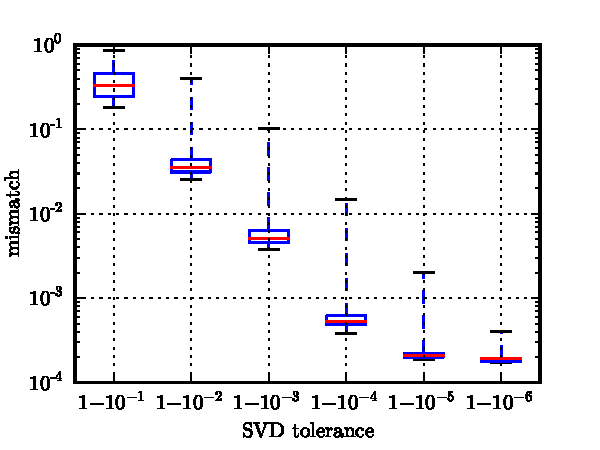
\includegraphics{figures/bw.pdf}
			(a) Mismatch versus \SVD\ tolerance
		\end{center}
	\end{minipage}
	\begin{minipage}[t]{0.5\textwidth}
		\begin{center}
			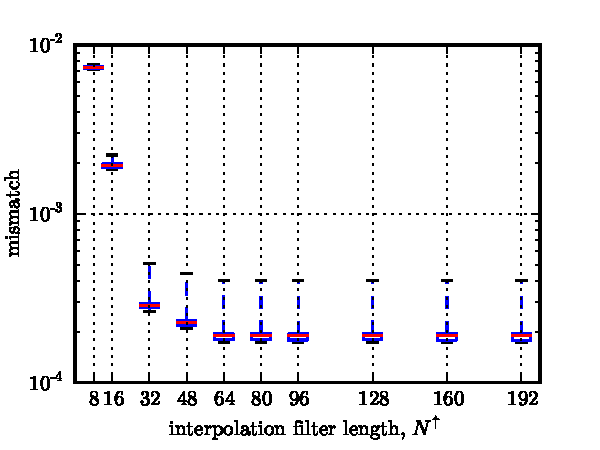
\includegraphics{figures/bw_resample.pdf}
			(b) Mismatch versus $N^\shortuparrow$
		\end{center}
	\end{minipage}
	\caption{\label{fig:bw}Box-and-whisker plot of mismatch between nominal
template bank and \lloid\ measured impulse responses.  The upper and lower boundaries of
the boxes show the upper and lower quartiles; the lines in the center denote the medians.
The whiskers represent the minimum and maximum mismatch over all templates.  In 
(a) the interpolation filter length is held fixed at $N^\shortuparrow = 192$, while
the \SVD\ tolerance is varied from $\left(1-10^{-1}\right)$ to $\left(1-10^{-6}\right)$.
In (b), the \SVD\ tolerance is fixed at $\left(1-10^{-6}\right)$ while $N^\shortuparrow$
is varied from 8 to 192 coefficients.}
\end{figure*}

\subsection{Lower bounds on computational cost compared to other methods}

We are now prepared to offer the estimated computational cost of filtering this
sub-bank of templates compared to other methods.  We used the results of the
previous subsections to set the \SVD\ tolerance at $\left(1-10^{-4}\right)$ and the
interpolation filter length to 16. Table \ref{table:flops} shows the computational cost
in \flops\ for this sub-bank.  Fort the \FD\ method, an \fft\ block size of $\fftblock = 
2 \tmpsamps$ is assumed, resulting in a latency of $\left(\tmpsamps f^0\right)$
seconds.  Both the \FD\ method and \lloid\ are five orders of magnitude faster than
the conventional \TD\ method.  However, the \FD\ method has a latency of over half of an
hour, whereas \lloid\ has no latency at all.
%
\begin{table}
\caption{Computational cost in \flops\ of the \TD\ method, the \FD\ method, and \lloid\ for the sub-bank described in section~\ref{sec:bank-setup}.}
\begin{center}
\begin{tabular}{lll}
\tableline\tableline
method & \flops\ & latency (s) \\
\tableline
time domain & $2.4\times10^{13}$ & 0 \\
frequency domain & $2.6\times10^8$ & 2201 \\
\lloid\ (this work) & $4.7\times10^8$ & 0 \\
\tableline
\end{tabular}
\end{center}
\end{table}

\subsection{Extrapolation of the computational cost to an Advanced \LIGO{} search}

Table~\ref{table:flops} shows that the \lloid\ method requires $\sim$$10^8$
\flops\ to cover a sub-bank comprising $\sim$$10^2$ out of the total $\sim$$10^5$
mass pairs.  Given that modern (ca. 2011) workstations can sustain computation
rates up to $\sim$$10^{10}$ \flops{}, and assuming that other regions of the
parameter space have similar computational scaling, an entire search could be
implemented with $\gtrsim$$10$ machines.  The lengths of templates does vary
over the parameter space; lower-mass templates are longer and would require
more computation to analyze while higher-mass templates are shorter and would
require less. However, we consider the estimates based on this sub-bank to be a
reasonable representation.

By comparison, using the \TD\ method to achieve the same latency costs
$\sim$$10^{13}$ \flops\ for this particular sub-bank, and so it would require
$\sim$$10^6$ present-day machines to search the full parameter space.
Presently, the \LIGO{} Data Grid consists of only $\sim$$10^4$ machines.


